\documentclass[14pt, a4paper]{article}
\usepackage{graphicx}
\usepackage[12pt]{extsizes}
\graphicspath{{pictures/}}
\DeclareGraphicsExtensions{.pdf,.png,.jpg}
\usepackage[utf8]{inputenc}
\usepackage[english,russian]{babel}
\usepackage{amssymb}
\usepackage{amsmath}
\usepackage{xcolor}
\usepackage{hyperref}
\definecolor{linkcolor}{rgb}{0, 0, 0} % цвет ссылок
\definecolor{urlcolor}{rgb}{0, 0, 0} % цвет гиперссылок
\renewcommand
\hypersetup{pdfstartview=FitH,  linkcolor=linkcolor,urlcolor=urlcolor, colorlinks=true}
\linespread{1}
\usepackage{xcolor}
\usepackage{geometry}  %поля
\geometry{left=2.5cm}
\geometry{right=1cm}
\geometry{top=2cm}
\geometry{bottom=2cm}

\begin{document}
	\begin{titlepage}
		\begin{center}
			\textbf{МИНИСТЕРСТВО ОБРАЗОВАНИЯ РЕСПУБЛИКИ БЕЛАРУСЬ}
		\end{center}
		\begin{center}
			\textbf{БЕЛОРУССКИЙ ГОСУДАРСТВЕННЫЙ УНИВЕРСИТЕТ}
		\end{center}
		\begin{center}
			\textbf{ФАКУЛЬТЕТ ПРИКЛАДНОЙ МАТЕМАТИКИ И ИНФОРМАТИКИ}
		\end{center}
		\begin{center}
			Кaфедрa теории вероятностей и мaтемaтической стaтистики
		\end{center}
		\vfill
		\begin{center}
			\large{\bf{Отчет о прохождении преддипломной практики}}
		\end{center}
		
		\vfill
		
		\begin{tabular}{p{80mm}p{90mm}}
			&
			студента 4 курса 7 группы\newline
			
			Джига Александра Олеговича\newline
			
			специальность "прикладная математика"\newline
			
			Руководитель практики:\newline
			
			\textit{Дудин Александр Николаевич}\newline
			
			доктор физико-мaтемaтических нaук, \newline профессор
			\vskip 1em
			
		\end{tabular}
		\vfill
		\vfill
		\begin{center}Минск 2019\end{center}
	\end{titlepage}
\setcounter{page}{2}
\begin{center}
	\section*{Реферат}
	\begin{flushleft}
		$\qquad$Ключевые слова: СИСТЕМА МАССОВОГО ОБСЛУЖИВАНИЯ,
		СИСТЕМА MAP|G|1, ПЕРЕХОДНЫЕ ВЕРОЯТНОСТИ, КРИТЕРИЙ
		ЭРГОДИЧНОСТИ, СТАЦИОНАРНОЕ РАСПРЕДЕНИЯ ВЕРОЯТНОСТЕЙ.\\
		Объектом исследования является система массового обслуживания типа
		$MAP|G|1$ с генерацией энергии. Цель работы – изучить систему, описать модель
		и исследовать ее поведение в различных случаях. Найдены переходные
		вероятности системы. Построена матрица переходных вероятностей. Найдено
		условие эргодичности.
	\end{flushleft}
	\begin{flushleft}
		$\qquad$Ключавыя словы: СIСТЭМА МАСАВАГА АБСЛУГОЎВАННЯ,
		СIСТЭМА MAP | G | 1, ПЕРАХОДНЫЯ IМАВЕРНАСЦI, КРЫТЭРЫЙ
		ЭРГАДЗIЧНАСЦI, СТАЦЫЯНАРНАЕ РАЗМЕРКАВАННЕ IМАВЕРНАСЦЕЎ.\\
		Аб’ектам даследавання з’яўляецца сiстэма масавага абслугоўвання тыпу
		$MAP|G|1$ з генерацыяй энергii. Мэта работы - вывучыць сiстэму, апiсаць мадэль
		i даследаваць яе паводзiны ў розных выпадках. Знойдзеныя пераходныя
		iмавернасцi сiстэмы. Пабудавана матрыца пераходных iмавернасцеў.
		Знойдзена ўмова эргадзічнасці.
	\end{flushleft}
	\begin{flushleft}
		$\qquad$ Key words: QUEUEING SYSTEM, MAP | G | 1 SYSTEM, TRANSITION
		PROBABILITIES, ERGODICITY CRITERION, STATIONARY DISTRIBUTION
		OF PROBABILITIES.\\
		The object of the study is a queuing system of the $MAP|G|1$ type with the
		generation of energy. The aim of the work is to study the system, describe the
		model and investigate its behavior in various cases. The transition probabilities
		of the system are found. A matrix of transition probabilities is constructed. The
		ergodicity condition is found.
		parameters.

	\end{flushleft}
\end{center}
\newpage
\tableofcontents

\newpage
	\large
	\begin{center}
		\textbf{ВВЕДЕНИЕ}\\
	\end{center}

	Математические модели систем массового обслуживания (СМО) широко применяются для исследования и оптимизации процессов в различных физических, экономических, производственных, административных, медицинских, военных и других системах. Объектом исследования в теории СМО являются ситуации, когда имеется некоторый ограниченный ресурс и множество запросов на удовлетворения потребности в этом ресурсе. Примерами могут служить кассы в магазинах, аэропортах, вокзалах и т.д.; терминалы в транспортных системах; банкоматы, инфокиоски и точки оплаты с использованием пластиковых карт; таблицы и индексы реляционных баз данных; ресурсы медицинских, экстренных и аварийных служб; средства радиолокации и противовоздушной обороны; авторизационные серверы в банках, контактные, справочные и информационные центры и т.д. Ограниченность ресурса и случайный характер потока запросов приводят к отказу или задержке в удовлетворении запросов. Стремление уменьшить вероятность этих отказов и длительность задержек и явилось побуждающим мотивом развития теории СМО. С точки зрения используемого математического аппарата, теория СМО может быть классифицирована как прикладная ветвь теории вероятностей, а более точно, теории случайных процессов. Классическая теория СМО основана на использовании известных результатов из теории цепей Маркова с непрерывным временем (и, в частности, теории процессов гибели и размножения) и дискретным временем, теории марковских, полумарковских, линейчатых и близких к ним процессов. Все эти процессы являются одномерными или двумерными (где вторая компонента является непрерывной, носит вспомогательных характер и предназначена для получения марковского процесса).
	
	\section{МАТЕМАТИЧЕСКАЯ МОДЕЛЬ СИСТЕМЫ MAP|G|1 С ГЕНЕРАЦИЕЙ ЭНЕРГИИ}
	\subsection{Математическая модель}
	Поступление единиц энергии подчинено пуассоновскому
	процессу с параметром $\gamma$. Запросы поступают $MAP$ - потоком под управлением
	неприводимой ЦМ с параметром $\nu_{t},\\ t\geq 0$, с непрерывным временем. Время пребывания цепи $\nu_{t}$ в
	некотором состоянии $\nu$ имеет показательное распределение с параметром
	$\lambda_{\nu}$. После того, как время пребывания процесса в этом состоянии
	истекло, с вероятностью $p_{l}(\nu, \nu')$ процесс $\nu_{t}$ переходит (перескакивает) в
	некоторое состояние $\nu'$ и генерируется группа из $l$ запросов, $l =0, 1$. При
	этом $p_{0}(\nu, \nu)$= = 0. Для $MAP$-потока невозможно определить считающую функцию как в стационарном пуассоновском(как безусловную вероятность), поскольку число запросов, поступивших за интервал времени длиной $t$ зависит от состояния управляющего
	процесса $\nu_{t}$, $t\geq $0, в момент начала этого интервала. Но можно вычислить
	вероятности $P_{\nu, \nu'}(l , t)$
	(за время $t$ поступит $l$ запросов и $\nu_{t} = \nu'$ при условии $\nu_{0} = \nu$).

	Вероятность поступления 0 запросов за время $t$ имеет вид $P(0, t) = e^{D_{0}t}$.  Здесь $D_{k}$ – квадратные матрицы порядка $W + 1$, элементы которых определяются следующим образом:

	$$(D_0)_{\nu,\nu'}=\left\{
	\begin{array}{rcl}-\lambda_\nu, &\nu=\nu',\\\lambda_\nu p_0(\nu,\nu'),
	&\nu\neq\nu',
	\end{array}\right.$$
	$$(D_k)_{\nu,\nu'}=\lambda_\nu p_k(\nu,\nu'), k\geq 1,
	$$
	$D(z) = D_{0} + D_{1}z$.\\
	 Запросы поступают 
	в прибор в порядке FIFO. Время обслуживания прибора имеет функцию
	распределения $B(t)$.\\
	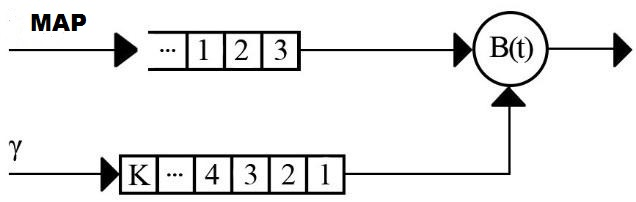
\includegraphics{img139}\\
	Для обслуживания одного запроса необходима одна единица энергия. Единица энергии
	берется сразу после того, как запрос поступит на обслуживание.  Если же буфер
	для хранения энергии пуст, то система переходит в режим ожидания
	до тех пор, пока не поступит единица энергии. Если буфер энергии заполнен,
	то поступающие единицы энергии теряются.\newpage
	\subsection {Необходимые обозначения}

Вероятность поступление в буфер $k$ единиц энергии за время $t$:

$\phi_{k}(t) = \frac{(\gamma t)^{k} }{k!} e^{-\gamma t}, k \geq 0$.

Вероятность поступление в буфер не менее $k$ единиц энергии за время $t$:

$\ \hat\phi_{k}(t) = \sum\limits_{i=k}^{\infty} \phi_{i}(t), k \geq 0$.

Матрица вероятностей поступления $i$ заявок и  $k$ единиц энергии за время обслуживания одной заявки:

$\ \Phi(i, k) =  \int\limits_{0}^{\infty} P(i,t)\phi_{k}(t)dB(t), i \geq 0, k \geq 0$.

 Матрица вероятностей поступления $i$ заявок и не менее $k$ единиц энергии за время обслуживания одной заявки:
 
$\ \hat\Phi(i, k) = \int\limits_{0}^{\infty}  P(i, t) \hat\phi_{k}(t)dB(t), i \geq 0, k \geq 0$.

Матрица вероятностей того, что за время отсутствия единиц энергии в буфере поступит $n$ запросов:

$\ N(n) = \int\limits_{0}^{\infty} P(n, t)\gamma e^{-\gamma t}dt$.

Матрица вероятностей того, что за время отсутствия запросов поступит $n$ единиц энергии:

$\ M(n) = \int\limits_{0}^{\infty} e^{D_{0}t}\phi_{n}(t)D_{1}dt = 
	\int\limits_{0}^{\infty} e^{D_{0}t}\frac{(\gamma t)^{n} }{n!} e^{-\gamma I t}D_{1}dt = \gamma^{n}(-D_{0} + + \gamma I)^{-(n+1)}D_{1}
$.

Матрица вероятностей того, что за время отсутствия запросов в буфере поступит не менее $m$ единиц энергии: 

$\ \hat M(m) = \sum\limits_{n=m}^{\infty} M(n)$.\\

Матрица $P(n, t)$ это матрица вероятности что за время ${t}$ поступит ${n}$
запросов.
Матрицы $P(n, t)$, ${n}$ > 1, в принципе, могут быть вычислены через матричную ПФ $P(z, t)$, имеющую вид $P(z, t) = e^{D(z)t}$, следюущим образом: 
$$
P(n,t)=\left. \frac{1}{n!} \frac{\partial^n P(z,t)}{\partial z^n}
\right|_{z=0}, \,n\geq 0.
$$
Однако, вычисление матриц $P(n,t)$ в аналитическом виде по этой формуле возможно только в редких случаях.
В общем виде они вычисляются с помощью процеду, основанной на идее униформизации марковского процесса, которая состоит в следующем.

Если $H$ – инфинитезимальный генератор ЦМ с непрерывным временем,
то справедливо представление:
$$
e^{Ht}=e^{ht(L-I)}=e^{-ht}e^{htL}=\sum_{j=0}^{\infty}e^{-ht}{(ht)^j\over
	j!}L^j,
$$
где 
$$
h=\max_{i=\overline{0,W}}(-H)_{ii},\ L=I+h^{-1}H.
$$

Матрица $L$ является матрицей одношаговых переходных вероятностей
некоторой вспомогательной ЦМ с дискретным временем. Весьма полезным свойством представления является мультипликативность членов суммы, представление их в виде произведения скалярной функции от
аргумента $t$ и матрицы, не зависящей от $t$.

Нетрудно видеть, что аналогичное разложение, с поправкой на то, что
$L$ - субстохастическая матрица, может быть применено к матричной экспоненте в случае, когда $H$ – матрица, у которой недиагональный элементы
неотрицательны, диагональные – отрицательны и суммы по строкам – отрицательны или равны нулю. В частности, такое разложение справедливо
для матричной экспоненты $e^{D_{0}t}$.

Обозначим $\tilde \theta=\max\limits_{i=\overline{0,W}}(-D_0)_{ii}$.
Тогда $P(0,t)=e^{D_0t}$ можно представить в виде
$$
P(0,t)=\sum_{j=0}^{\infty}e^{-\tilde \theta t}{(\tilde \theta t)^j\over
	j!}K_0^{(j)},
$$
где
$$K_0^{(j)}=(I+\tilde \theta^{-1}D_0)^j.
$$
По аналогии, будем искать остальные матрицы $P(n, t), n \ge 1$, в виде
$$
P(n,t)= \sum_{j=0}^{\infty}e^{-\tilde \theta t}{(\tilde \theta
	t)^j\over j!}K_n^{(j)},\; n \ge 1,
$$
где $K_n^{(j)},\; n \ge 1, j \ge 0,$ -- некоторые матрицы.
Матрицы $K_n^{j}$ удовлетворяют следующей системе рекуррентных соотношений: 
$$
K_0^{(0)}=I,\ K_n^{(0)}=O,\ n\ge 1,
$$ $$
K_0^{(j+1)}=K_0^{(j)}(I+\tilde \theta^{-1}D_0),
$$ $$
K_n^{(j+1)}=\tilde
\theta^{-1}K_{n - 1}^{(j)}D_{1}+K_n^{(j)}(I+\tilde
\theta^{-1}D_0),\; n \ge 1,\; j \ge 0.
$$ 
Усечение бесконечной суммы в можно
произвести после того, как член суммы окажется по норме меньше наперед заданного малого положительного числа. Следует также учитывать, что первые несколько значений при вычислении матриц $K_n^{(j)}$ могут равняться нулевым матрицам. 
\subsection{Переходные вероятности}
Данный процесс является немарковским. Для его исследования применим метод вложенных ЦМ. Будем
рассматривать поведение СМО $(i_{t}, k_{t})$, в моменты $t_{n}, \; n\geq1$ окончания  обслуживания запросов, а именно, рассмотрим процесс
$\epsilon_{n} = \left\{i_{n}, k_{n}, \nu_{n}\right\}$ - трехмерный процесс, где $i_{n} = i_{t_{n+0}},\; k_{n} = k_{t_{n-0}},\; \nu_{n} = \nu_{t_{n}}.$
Данный процесс является трехмерной цепью Маркова. Введем матрицу $$P\left\{(i,k) \rightarrow (j, k')\right\},$$ ($\nu\nu'$)-й элемент которой есть вероятность одношагового перехода: $$P\left\{ (i ,k, \nu) \rightarrow (j, k', \nu') )\right\} =$$  $$=P\left\{i_{n+1} = j, k_{n+1} = k', \nu_{n+1} = \nu' |i_{n} = i, k_{n} = k, \nu_{n} = \nu \right\}$$
Введем стационарные вероятности $$ \pi(i, k, \nu') = \lim_{n -> \infty}P\left\{i_{n} = i, k_{n} = k, \nu_{n} = \nu\right\},$$ $$ i \geq 0, k \in [0, K], \nu \in [0, W],$$ которые объединим в вектора $$\boldsymbol{\pi}(i, k) = (\pi(i, k, 0),..., \pi(i, k, W), k \in [0, K],$$ которые, в свою очередь, образуют вектор стационарных вероятностей:
$$\boldsymbol{\pi}_{i} = (\boldsymbol{\pi}(i, 1),..., \boldsymbol{\pi}(i, K)), i \geq 0.$$
Нахождение переходных вероятностей в частных случаях проводится путем анализа поведения цепи Маркова между моментами $t_{n}$ и $t_{n+1}$ и использования формулы полной вероятности.$\\$ 
\textbf{Лемма}\\
Матрицы $P\left\{(i,k) \rightarrow (j, k')\right\}$ вычисляются следующим образом:

$$P\left\{(0, 0) \to (j, k' ) \right\}=M(0)\sum\limits_{n = 0}^{j}N(n)\Phi(j-n, k') $$ $$ + N(0)\sum\limits_{m = 0}^{k'}M(m)\Phi(j, k' - m), j\geq 0,\; k'= \overline{0,K-2};$$

$$P\left\{(0, 0) \to (j,K-1 ) \right\}=M(0)\sum\limits_{n = 0}^{j}N(n)\Phi(j-n, K-1) $$ $$ + N(0)[\sum\limits_{m = 0}^{K-1}M(m)\Phi(j, K-1 - m)+\hat {M}(K) \Phi(j, 0)], j\geq 0;$$

$$P\left\{(0, 0) \rightarrow (j, K) \right\}=M(0)\sum\limits_{n = 0}^{j}N(n)\hat\Phi(j-n, K) $$$$+ N(0)(\sum\limits_{m = 0}^{K-1}M(m)\hat\Phi(j, K - m) + \hat M(K)\hat \Phi(j, 1)),\; j\geq 0.$$

$$P\left\{(0, k) \to (j, K-1) \right\}=\sum\limits_{m = 0}^{K-k}M(m)\Phi(j,K-k - m)+ $$ $$+
\hat{M}(K-k+1)\Phi(j,0), j\geq 0,\; k=\overline{1,K};$$

$$P\left\{(0, k) \rightarrow (j, k') \right\}=\sum\limits_{m = 0}^{k'-k+1}M(m)\Phi(j,k' - k + 1 - m),$$ $$ j\geq 0,\; k=\overline{1,K}, k' =\overline{k-1,K-2}.$$	

$$P\left\{(0, k) \rightarrow (j, K)\right\}=\sum\limits_{m = 0}^{K-k}M(m) \hat \Phi(j, K - k + 1 - m) + $$ $$\hat M(K - k + 1)\hat \Phi(j, 1),\; j\geq 0,\; k =\overline{1,K}.$$

$$P\left\{(i, 0) \rightarrow (j, k') \right\}= \sum\limits_{n = 0}^{j - i + 1}N(n)\Phi(j - i + 1 - n, k'),$$ $$ i\geq 1,\; j \geq i-1,\; k' =\overline{0, K-1}. $$

$$P\left\{(i, 0) \rightarrow (j, K) \right\}=\sum\limits_{n = 0}^{j - i + 1}N(n)\hat \Phi(j - i + 1 - n, K),\; i \geq 1,\; j\geq i-1. $$


$$P\left\{(i, k) \rightarrow (j, k') \right\} =\Phi(j - i + 1, k' - k+1),$$ $$ i \geq 1,\; j\geq i-1,\; k' =\overline{k-1, K-1}, k=\overline{1,K}.$$

$$P\left\{(i, k) \rightarrow (j, K)\right\}= \hat \Phi(j - i + 1, K - k+1),\; i \geq 1,\; j\geq i-1, $$ $$ k=\overline{1,K}.$$

\section{ПОСТРОЕНИЕ МАТРИЦЫ ПЕРЕХОДНЫХ ВЕРОЯТНОСТЕЙ}

\subsection{Матрица вероятностей переходов}
Матрица $P$ вероятностей одношаговых переходов рассматриваемого
процесса имеет следующую форму $P = (P_{i,j})i,j \geq 0$. Можно показать, что
матрицы $P_{i,j}$ не зависят от $i$ и $j$, а зависят только от $j - i$. Тогда
обозначим матрицы $(P_{i,j})i=0,\; j \geq 0$  как $ V_{j}$, элементами которых будут переходные
вероятности $P\left\{(0, k) \rightarrow (j, k') \right\}$, где $ k, k' \in [0, K]$. Заметим, что для $i \geq 1$ выполняется следующее:\\
$(P_{i, j-i+1},\: j\geq 0) = (P_{ij}),\: j \geq 0 .\\$
Матрицы $P_{i,i + j - 1}\: i\neq 0,\: j \geq 0,$ в свою очередь, обозначим как $Y_{j},$ элементами которых
будут переходные вероятности $P\left\{(1, k) \rightarrow (j, k') \right\}$ , где $ k, k' \in [O,K]$. Матрица
вероятностей одношаговых переходов $P$ имеет следующую структуру: \\
$P=\begin{bmatrix}
V_{0} & V_{1} & V_{2} & V_{3} & V{_4} & \ldots\\
Y_{0} & Y_{1} & Y_{2} & Y_{3} & Y{_4} & \ldots\\
0 & Y_{0} & Y_{1} & Y_{2} & Y_{3} & \ldots\\
0 & 0 & Y_{0} & Y_{1} & Y_{2} & \ldots\\
\vdots & \vdots & \vdots & \vdots & \vdots & \ddots\\
\end{bmatrix}$\\
Матрицу, имеющие такую структуру, называют блочной верхне-Хессенберговой. Величина скачка вниз компоненты $i_{n}$ за один шаг не превосходит
единицы.

\subsection{Вид матриц $V_{j}$}
Матрицы $V_{j}$ имеют следующий вид: \\
$\begin{bmatrix}
v^{j}_{00} & v^{j}_{01} & v^{j}_{02} & v^{j}_{03} & \ldots & v^{j}_{0K}\\
v^{j}_{10} & v^{j}_{11}& v^{j}_{12} & v^{j}_{13}& \ldots& v^{j}_{1K}\\
0& v^{j}_{21}& v^{j}_{22}& v^{j}_{23}& \ldots & v^{j}_{2K}\\
0& 0& v^{j}_{32}& v^{j}_{33}& \ldots &v^{j}_{3K}\\
\vdots & \vdots & \vdots & \vdots & \ddots & \vdots\\
0 & 0 & 0 & 0 & \ldots  & v^{j}_{KK}\\
\end{bmatrix}$\\\\
Где $v^{j}_{kk'}$ находятся следующим образом:\\
$a)\;v^{j}_{0k'} = P\left\{(0, 0) \rightarrow (j, k') \right\} = M(0)\sum\limits_{n = 0}^{j}N(n)\Phi(j-n, k') +  \\ + N(0)\sum\limits_{m = 0}^{k'}M(m)\Phi(j, k' - m), j\geq 0,\; k'= \overline{0,K-1},\\
b)\;v^{j}_{kk'} = P\left\{(0, k) \rightarrow (j, k') \right\} = \sum\limits_{m = 0}^{k'-k+1}M(m)\Phi(j,k' - k + 1 - m), \\ j\geq 0,\; k=\overline{1,K}, k' =\overline{k-1,K-1},\\
c)\;v^{j}_{kK} = P\left\{(0, k) \rightarrow (j, K) \right\} = \sum\limits_{m = 0}^{K-k}M(m) \hat \Phi(j, K - k + 1 - m) + \\ + \hat M(K - k + 1)\hat \Phi(j, 1),\; j\geq 0,\; k =\overline{1,K}.\\
d)\;v^{j}_{0K} = P\left\{(0, 0) \rightarrow (j, K) \right\}=M(0)\sum\limits_{n = 0}^{j}N(n)\hat\Phi(j-n, K) +\\ + N(0)(\sum\limits_{m = 0}^{K-1}M(m)\hat\Phi(j, K - m) + \hat M(K)\hat \Phi(j, 1)),\; j\geq 0., \\
e)\;v^{j}_{0(K - 1)} = P\left\{(0, 0) \to (j,K-1 ) \right\}=M(0)\sum\limits_{n = 0}^{j}N(n)\Phi(j-n, K-1) \\ + N(0)[\sum\limits_{m = 0}^{K-1}M(m)\Phi(j, K-1 - m)+\hat {M}(K) \Phi(j, 0)], j\geq 0,\\
f)\;v^{j}_{k(K - 1)} = P\left\{(0, k) \to (j, K-1) \right\}=\sum\limits_{m = 0}^{K-k}M(m)\Phi(j,K-k - m)+ \\+
\hat{M}(K-k+1)\Phi(j,0), j\geq 0,\; k=\overline{1,K}\\
$
Проанализировав вид $v^{j}_{kk'}$ сделаем вывод, что, начиная со второй строки,
элементы не зависят от $k$ и $k'$, а зависят только $k' - k$.
\subsection{Вид матриц $Y_{j}$}
Матрицы $Y_{j}$ имеют следующий вид: \\
$\begin{bmatrix}
y^{j}_{00} & y^{j}_{01}& y^{j}_{02}& y^{j}_{03}& \ldots & y^{j}_{0K}\\
y^{j}_{10} & y^{j}_{11}& y^{j}_{12}& y^{j}_{13}& \ldots & y^{j}_{1K}\\
0 & y^{j}_{21}& y^{j}_{22}& y^{j}_{23}& \ldots & y^{j}_{2K}\\
0& 0& y^{j}_{32}& y^{j}_{33}& \ldots & y^{j}_{3K}\\
\vdots & \vdots & \vdots & \vdots & \ddots & \vdots\\
0 & 0 & 0 & 0 & \ldots & y^{j}_{KK}\\
\end{bmatrix}$\\ \\
Где $y^{j}_{kk'}$ находятся следующим образом:\\

$a)P\left\{(i, 0) \rightarrow (j, k') \right\}= \sum\limits_{n = 0}^{j - i + 1}N(n)\Phi(j - i + 1 - n, k'),$$ $$ i\geq 1,\; j \geq i-1,\; k' =\overline{0, K-1}. $

$b)P\left\{(i, 0) \rightarrow (j, K) \right\}=\sum\limits_{n = 0}^{j - i + 1}N(n)\hat \Phi(j - i + 1 - n, K),\; i \geq 1,\; j\geq i-1. $


$c)P\left\{(i, k) \rightarrow (j, k') \right\} =\Phi(j - i + 1, k' - k+1),$$ $$ i \geq 1,\; j\geq i-1,\; k' =\overline{k-1, K-1}, k=\overline{1,K}.$

$d)P\left\{(i, k) \rightarrow (j, K)\right\}= \hat \Phi(j - i + 1, K - k+1),\; i \geq 1,\; j\geq i-1, $$ $$ k=\overline{1,K}.$\\
Проанализировав вид $y^{j}_{kk'}$ сделаем вывод, что, начиная со второй строки,
элементы не зависят от $k$ и $k'$, а зависят только $k' - k$.
\section{СТАЦИОНАРНОЕ РАСПРЕДЕЛЕНИЕ ВЕРОЯТНОСТЕЙ}
\subsection{Критерий эргодичности системы}
Условие эргодичности можно трактовать следующим образом - 
условие, при котором система способна уменьшать число заявок в системе,
когда она перегружена, т.е. среднее число заявок, поступающих за время
обслуживания одной заявки, должно быть меньше единицы.\\
Введем матричные ПФ $V(z) = \sum\limits_{i = 0}^{\infty}V_{i}z^{i}$, $\;Y(z) = \sum\limits_{i = 0}^{\infty}Y_{i}z^{i}$, где $V_{j} = P_{0,i+j-1} и Y_{j} = P_{i,i+j-1}$\\
$Y(z) = \sum\limits_{j = 0}^{\infty}Y_{j}z^{j} =  \int\limits_{0}^{\infty}\sum\limits_{j = 0}^{\infty}z^{j}P(j, t)\frac{(\gamma t)^{k} }{k!}e^{-\lambda t}dB(t)$ =\\
$=\int\limits_{0}^{\infty}e^{D(z)t}\phi_{k}(t)dB(t)$, где $D(z) = D_{0} + D_{1}z$\\
\textbf{Теорема}\\
Пусть ЦМ $\epsilon_{n} = \left\{i_{n}, k_{n}, \nu_{n}\right\}$, с матрицей переходных вероятностей P является неприводимой и апериодической, матрицы $Y(1)$ и $V(1)$ являются стохастическими и неприводимыми и выполняются неравенства $V'(1) < \infty$ и $Y'(1) < \infty$. Для того, чтобы ЦМ $\epsilon_{n},\; n\geq 1$, была эргодичной, необходимо и достаточно, чтобы выполнялось неравенство:\\
$$[det(zl - Y(z))]'_{z=1} > 0     \eqno(1)\\$$
\textbf{Следствие}\\
Неравенство (1) эквивалентно следующему неравенству:\\
$\vec{y}\sum\limits_{k = 1}^{\infty}kY_{k}(1)e\;<\;1$,\\
где вектор $\vec{y}$ удовлетворяет системе уравнений:\\
$
\begin{cases}
\vec{y}\sum\limits_{k = 0}^{\infty}Y_{k}(1) = \vec{y}\\
\vec{y}e = 1.
\end{cases}\\
$
Пусть вектор $y$ имеет вид \\
$$y = \theta\otimes u\eqno(2)$$
где ${\theta}$ - вектор стационарного распределения процесса $MAP$ $\nu_t,\,t\geq0,$ и $u= (u_{1}, u_{2}, . . . , u_{K})$.
Найдем вектор u. Компоненты вектора u
удовлетворяют следующей системе алгебраических уравнений:\\
$
\begin{cases}
u_{k} = u_{0}\phi_{k} + \sum\limits_{s=1}^{k+1}u_{s}\phi_{k + 1 - s}, k = \overline{0, K-1},\\
u_{K} = u_{0}\hat\phi{k} + \sum\limits_{s=1}^{K}u_{s}\phi_{K + 1 - s}.
\end{cases}\\
$
Решим эту систему, представив $u_{k}$ следующим образом:\\
$
\begin{cases}
	u_{k} = u_{0}\psi_{k}\\
	u_{0} = (\sum\limits_{k=0}^{K}\psi_{k})^{-1},
\end{cases}\\
$
Где $\psi_{k + 1}$:\\
$\psi_{k+1}\; =\;(\psi_{k} - \phi_{k} - \sum\limits_{s=1}^{k}\psi_{s}\phi_{k + 1 - s})\phi_{0}^{-1}, k = \overline{0, K-1}, \psi_{0} = 1 $\\
После подстановки $u$ и $y$ получаем условие эргодичности:\\
$\lambda T + u_{0}  \frac{\lambda}{\gamma}\; <\; 1$,\\
где $T$ это время обслуживания одной заявки.\\
Условие существования стационарного режима в системе совпадает с условием
эргодичности вложенной цепи Маркова. 
\begin{flushleft}\subsection{Матрично-аналитический метод для нахождения стационарного распределения вероятностей цепи Маркова (метод М. Ньютса)}\end{flushleft}

Краеугольным понятием в подходе М. Ньютса является понятие фундаментального периода. Фундаментальный период — это интервал времени с момента, когда значение счетной компоненты равно $i$, до первого момента, когда значение этой компоненты станет равным $i - 1$, $i \geq 1$. Из определения ЦМ типа $MAP|G|1$ следует, что длина фундаментального периода не зависит от значения $i$. 

Обозначим $G(z)$ матричную ПФ, $(k, k')$-й элемент которой есть ПФ числа переходов, осуществленных ЦМ за фундаментальный период, который закончился, когда значение конечной компоненты есть $k'$ при условии, что в момент начала фундаментального периода значение конечной компоненты равнялось $k$; $k, k' = \overline{0, K}$ . Используя факты из теории марковских процессов восстановления, можно показать, что матрица $G(z)$ удовлетворяет уравнению

\begin{equation}
\label{eq5}
G(z) = z \sum\limits_{j = 0}^{\infty} Y_j G^j(z).
\end{equation}

Обозначим через $G^{(i)}$ матрицу вероятностей переходов компоненты $k_n$ за время первого достижения первой компонентой $i_n$ значения $i$, начиная с $i + 1$.

Используя формулу полной вероятности, нетрудно убедиться, что матрицы $G^{(i)}, i \geq 0$, удовлетворяют уравнениям

\begin{equation}
\label{eq6}
G^{(i)} = P_{i + 1, i} + \sum\limits_{l = i + 1}^{\infty} P_{i + 1, l} G^{(l - 1)} G^{(l - 2)} \ldots G^{(i)}, i \geq 0.
\end{equation}

Учитывая квазитеплицевость рассматриваемой ЦМ, можно заключить, что матрицы $G^{(i)}, i \geq 0$, не зависят от $i$. Пусть все они равны некоторой матрице $G$. Тогда из (\ref{eq6}) можно заключить, что матрица $G$, удовлетворяет уравнению 

\begin{equation}
\label{eq7}
G = \sum\limits_{j = 0}^{\infty} Y_j G^j.
\end{equation}

Отметим, что уравнение (\ref{eq5}) автоматически следует из уравнения (\ref{eq7}), поскольку из определения матриц $G$ и $G(z)$ следует, что $G(1) = G$.

Обозначим через $\pi_i, i \geq 0$, векторы стационарных вероятностей исходной ЦМ $\xi_n, n \geq 1$.

\begin{equation}
\label{eq8}
\pi_j = \sum\limits_{i = 0}^{j} \pi_i \overline{P}_{i, j}, i \geq 0, 
\end{equation}

где матрицы $\overline{P}_{i, j}$ задаются уравнениями

\begin{equation}
\label{eq9}
\overline{P}_{i, j} = P_{i, j} + \sum\limits_{l = j + 1}^{\infty} P_{i, l} G^{l - j}, j \geq i. 
\end{equation}

Из (\ref{eq8}) следует, что векторы $\pi_i, i \geq 0$, стационарных вероятностей можно представить в виде

\begin{equation}
\label{eq10}
\pi_i = \pi_0 \Phi_i, i \geq 0, 
\end{equation}

где матрицы $\Phi_i, i \geq 0$ удовлетворяют рекуррентным соотношениям

\begin{equation}
\label{eq11}
\Phi_0 = I, \Phi_l = \left(\overline{P}_{0, l} + \sum\limits_{i = 1}^{l - 1} \Phi_i \overline{P}_{i, l}\right) \left(I - \overline{P}_{l, l}\right)^{-1}, l \geq 1.
\end{equation}

Соотношения (\ref{eq10}) определяют векторы $\pi_i, i \geq 0$, стационарных вероятностей с точностью до неизвестного пока вектора $\pi_0$. Этот вектор можно вычислить через аппарат векторных ПФ или по формуле (\ref{eq12}). Однако, предположим еще одну процедуру для подсчета вектора $\pi_0$.

Из уравнений (\ref{eq8}) при $j = 0$ получаем:

\begin{equation}
\label{eq12}
\pi_0(I - \overline{P}_{0, 0}) = 0. 
\end{equation}

Домножением соотношения (\ref{eq9}) справа на вектор $e$ несложно убедиться, что матрица $\overline{P}_{0, 0}$ - стохастическая. По построению эта матрица является неприводимой, поэтому ранг системы (\ref{eq12}) на единицу меньше размерности вектора $\pi_0$. Значит, система (\ref{eq12}) определяет вектор $\pi_0$ с точностью до некоторой константы. Следовательно, если нам удастся получить еще одно, неоднородное, уравнение для компонент вектора $\pi_0$, то полученнная система будет иметь единственное решение. Такое уравнение легко получается из (\ref{eq10}) и условия нормировки и имеет вид: 

\begin{equation}
\label{eq13}
\pi_0 \sum\limits_{i = 0}^{\infty} \Phi_i e = 1. 
\end{equation}

Подводя итог, сформулируем следующий алгоритм нахождения векторов $\pi_i, i \geq 0$, стационарных вероятностей:

\vspace{10pt}
\begin{enumerate}
	\item Находим матрицу $G$ как решение нелинейного матричного уравнения (\ref{eq7}).
	\item Вычисляем матрицы $\overline{P}_{i, l}$ по формулам (\ref{eq9}).
	\item Вычисляем матрицы $\Phi_l$ по рекуррентным формулам (\ref{eq11}).
	\item Находим вектор $\pi_0$ как единственное решение системы (\ref{eq12}), (\ref{eq13}).
	\item Ищем необходимое число векторов $\pi_i$ по формулам (\ref{eq10}).
\end{enumerate}
\pagebreak

\begin{flushleft}
	\section{АНАЛИЗ ХАРАКТЕРИСТИК ПРОИЗВОДИТЕЛЬНОСТИ СИСТЕМЫ}
\end{flushleft}
\setcounter{equation}{0}
\setcounter{figure}{0}
\setcounter{table}{0}

\subsection{Необходимые обозначения}
$n$ - количество векторов $\pi_{i}$. \\
$\pi_i = (\pi(i, 0), \pi(i, 1), \ldots, \pi(i, K)).$
\\
Среднее количество запросов в системе:
$$L = \sum\limits_{i = 0}^{n} i \pi_i e,$$
Среднее количество единиц энергии в буфере:
$$N =\sum\limits_{i = 0}^{n} \sum\limits_{k = 1}^{K} k \pi_{i}(k)e,$$
Вероятность отсутствия запросов в системе:
$$P_0^{custom} = \pi_0 e.$$
Вероятность отсутствия единиц энергии в буфере:
$$P_0^{energy} = \sum\limits_{i = 0}^{n} \pi_{i}(0)e.$$
Вероятность простоя системы по причине отсутствия единиц энергии в буфере:
$$P_{idle} = \sum\limits_{i = 1}^{n} \pi_{i}(0)e,$$.

\subsection{Численные характеристики системы}
Рассмотрим $MAP$-поток, который определяется матрицами $D_{0}$ и $D_{1}$, имеет среднюю интенсивность $\lambda = 0.4$ и $\gamma = 0.3$. Коэффициент корреляции $c_{cor} = 0.1724$, ${c_{var}=14.33}$.
\\

$D_{0} = \begin{pmatrix}
-0.405780& 0\\
0& -0.013173
\end{pmatrix}$,
$D_{1} = \begin{pmatrix}
0.403080& 0.002700\\
0.007338& 0.005835 
\end{pmatrix}$

\subsection{Среднее количество запросов в системе}
График $L$ для значений $k$ $($от $1$ до $K$ с шагом $1)$ и  $T$ $($от $0.5$ до $T$  с шагом $0.5)$.

\begin{figure}[h]
	\center{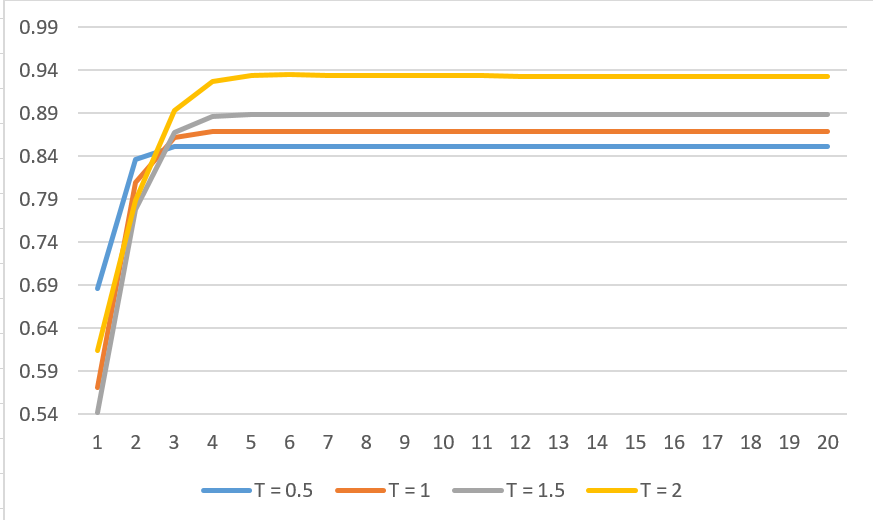
\includegraphics[width=1\linewidth]{11.png}}
	\caption{Среднее количество запросов в системе}
	\label{ris2}
\end{figure}


Среднее количество запросов в системе увеличивается по мере возрастания времени обслуживания. \pagebreak

\textbf{Входные данные:}


$K: 1, 2, 3, \ldots, 20$

$T: 0.5, 1.0, 1.5, 2$

$Accuracy: 0.001$
\\
\begin{figure}[h]
	\center{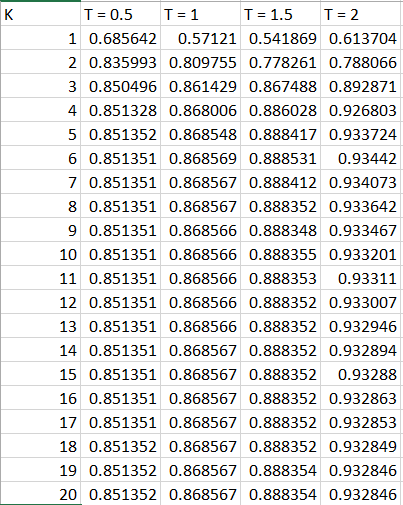
\includegraphics[scale=1.0]{1.png}}
\end{figure}
\pagebreak

\begin{flushleft}\subsection{Среднее количество единиц энергии в буфере}\end{flushleft}
График $N$ для значений $k$ $($от $1$ до $K$ с шагом $1)$ и  $T$ $($от $0.5$ до $T$  с шагом $0.5)$.

\begin{figure}[h!]
	\center{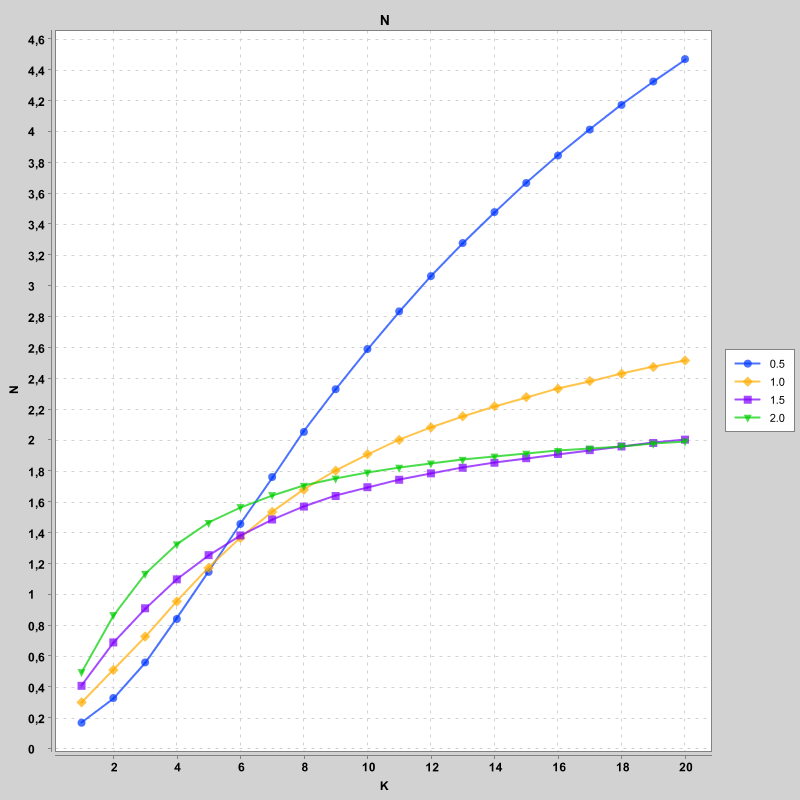
\includegraphics[width=1\linewidth]{12.png}}
	\caption{Среднее количество единиц энергии в буфере}
	\label{ris3}
\end{figure}

Среднее количество единиц энергии в буфере увеличивается с возрастанием времени обслуживания в системе. 
\pagebreak

\textbf{Входные данные:}


$K: 1, 2, 3, \ldots, 20$

$T: 0.5, 1.0$

$Accuracy: 0.001$

\begin{figure}[h]
	\center{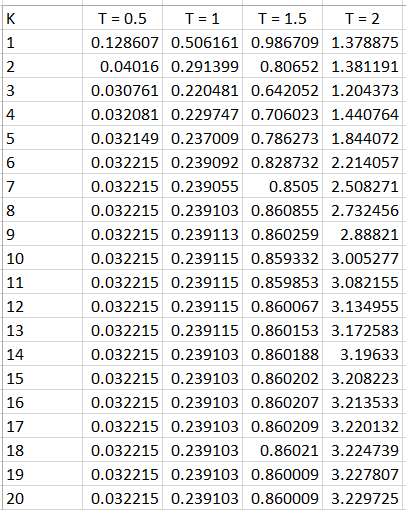
\includegraphics[scale=1]{2.png}}
\end{figure}

\pagebreak

\subsection{Вероятность отсутствия запросов в системе}
График $P_0^{custom}$ для значений $k$ $($от $1$ до $K$ с шагом $1)$ и  $T$ $($от $0.5$ до $T$  с шагом $0.5)$.
\begin{figure}[h!]
	\center{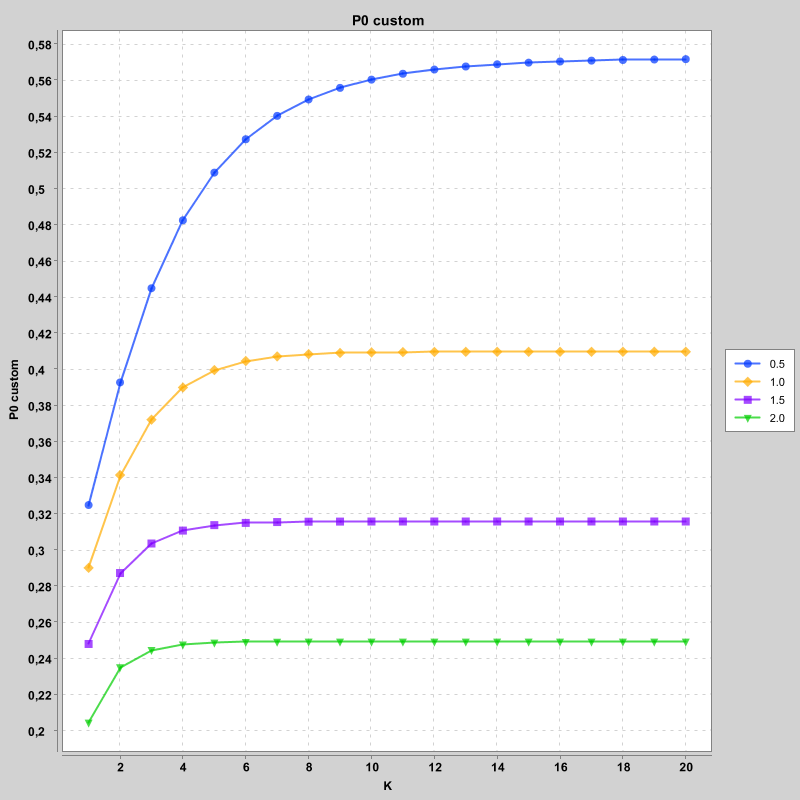
\includegraphics[width=1\linewidth]{13.png}}
	\caption{Вероятность отсутствия запросов в системе}
	\label{ris4}
\end{figure}


Вероятность отсутствия запросов в системе ведет себя довольно непредсказуемо, по графику видно, что она меньше всего при наименьшем времени обслуживания, возможно не хватает энергии.

\pagebreak
\textbf{Входные данные:}

$\lambda: 0.4$

$\gamma: 0.3$

$K: 1, 2, 3, \ldots, 20$

$T: 0.5, 1.0$

$Accuracy: 0.001$

\begin{figure}[h]
	\center{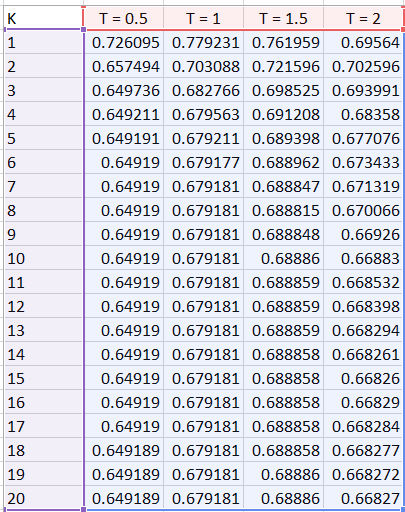
\includegraphics[scale=1]{3.png}}
\end{figure}
\pagebreak

\subsection{Вероятность отсутствия единиц энергии в буфере}
График $P_0^{energy}$ для значений $k$ $($от $1$ до $K$ с шагом $1)$ и  $T$ $($от $0.5$ до $T$  с шагом $0.5)$.

\begin{figure}[h!]
	\center{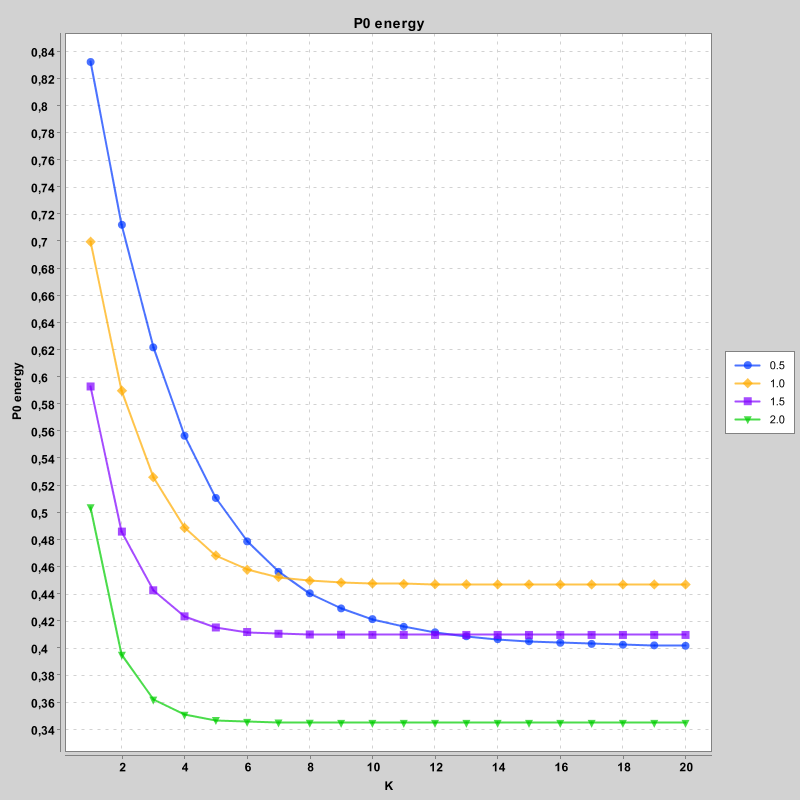
\includegraphics[width=1\linewidth]{14.png}}
	\caption{Вероятность отсутствия единиц энергии в буфере}
	\label{ris5}
\end{figure}

Вероятность отсутствия единиц энергии в буфере увеличивается по мере уменьшения времени обслуживания заявок системой. 

\pagebreak
\textbf{Входные данные:}

$\lambda: 0.4$

$\gamma: 0.3$

$K: 1, 2, 3, \ldots, 20$

$T: 0.5, 1.0$

$Accuracy: 0.001$

\begin{figure}[h]
	\center{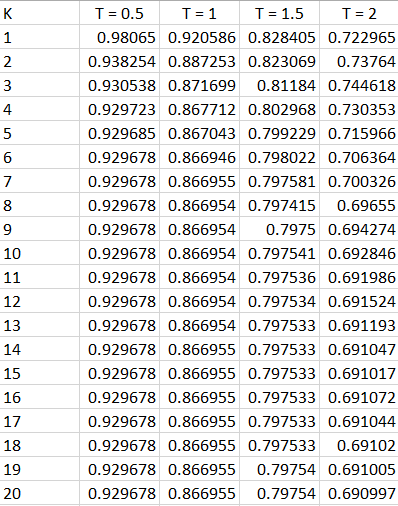
\includegraphics[scale=1]{4.png}}
\end{figure}

\pagebreak
\begin{flushleft}\subsection{Вероятность простоя системы по причине отсутствия единиц энергии в буфере}\end{flushleft}
График $P_{idle}$ для значений $k$ $($от $1$ до $K$ с шагом $1)$ и  $T$ $($от $0.5$ до $T$  с шагом $0.5)$.
\begin{figure}[h!]
	\center{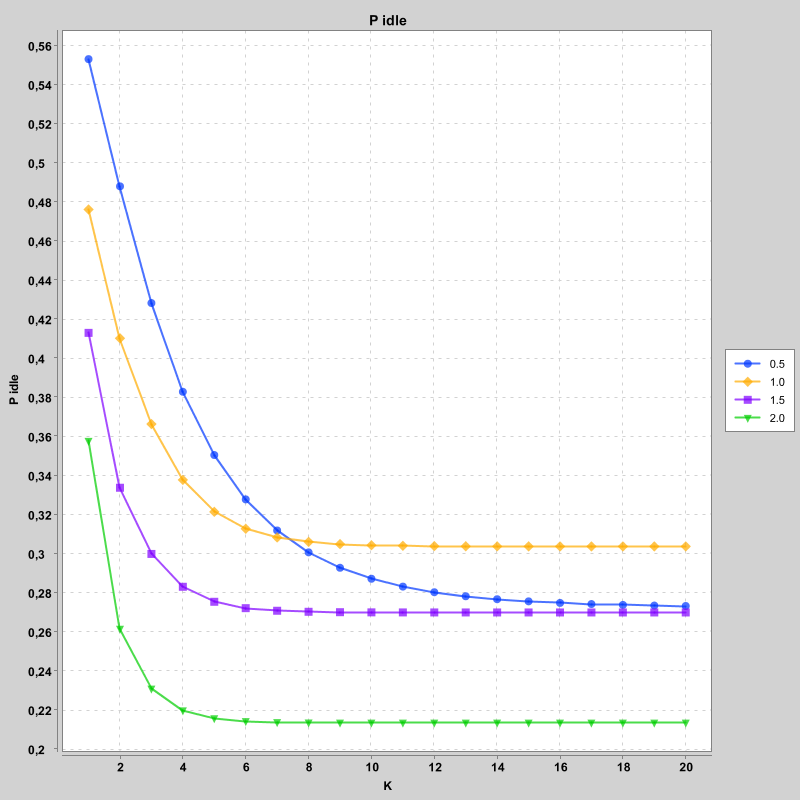
\includegraphics[width=1\linewidth]{15.png}}
	\caption{Вероятность простоя системы по причине отсутствия единиц энергии в буфере}
	\label{ris6}
\end{figure}

Вероятность простоя системы по причине отсутствия единиц энергии в буфере возрастает с уменьшением времени обслуживания. Другими словами - единицы энергии потребляются быстрее, что приводит к увеличению шанса простоя системы.

\pagebreak

\textbf{Входные данные:}

$\lambda: 0.4$

$\gamma: 0.3$

$K: 1, 2, 3, \ldots, 20$

$T: 0.5, 1.0$

$Accuracy: 0.001$



\begin{figure}[h]
	\center{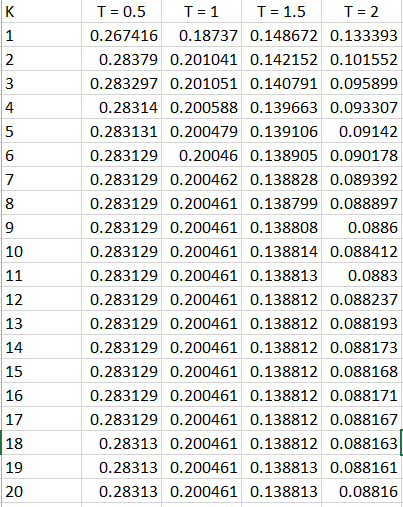
\includegraphics[scale=1]{5.png}}
\end{figure}
\pagebreak

\subsection{Вывод по итогам анализа характеристик производительности}

Путем сравнения характеристик производительности и выявления особенностей поведения системы можно повысить ее эффективность, повлияв на определенные параметры. Стоит отметить, что увеличение объема буфера энергии далеко не всегда способствует улучшению значения соответствующей характеристики т.к., начиная с определенного значения $K$, изменения достаточно малы и это экономически нецелесобразно, т.к не оказывает существенного влияния на работу системы.

Стоит добавить, что при исследовании системы при значениях $T > 2$ условие эргодичности начинает выполняться только для достаточно больших значений $K$.

\pagebreak

	\center{\section*{ЗАКЛЮЧЕНИЕ}}

\addcontentsline{toc}{section}{ЗАКЛЮЧЕНИЕ}

\begin{flushleft}
	В процессе выполнения курсовой работы:
	\begin{enumerate}
		\item Исследована система массового обслуживания типа $MAP|G|1$. Найдены вероятности одношаговых переходов, а так же построена матрица переходных вероятностей. Проверено выполнение условия эргодичности и на основе этого найдено стационарное распределение вероятностей.
		\item Разработана программная реализация предложенного метода нахождения стационарного распределения вероятностей на языке программирования Java.
		\item На основе программной реализации метода нахождения стационарного распределения вероятностей найдены характеристики производительности искомой системы. Произведен их анализ и сделаны выводы. 
	\end{enumerate}
\end{flushleft}
\newpage
\begin{thebibliography}{20}
	\bibitem{kd}
	Klimenok  V.I.,   Dudin A.N.  Multi-dimensional asymptotically quasi-Toeplitz
	Markov chains and their application in queueing theory // Queueing
	Systems. 2006. V. 54. P. 245-259.
\end{thebibliography}
\end{document}
